\documentclass[12pt,a4paper]{article}
\usepackage{amsmath, amssymb, geometry, booktabs, xcolor, hyperref,
            listings, pgfplots, tcolorbox, enumitem, fancyhdr, tikz, array}
\geometry{margin=2.5cm}
\pgfplotsset{compat=1.18}
\tcbuselibrary{skins, breakable}

%--- tcolorbox environments ---
\newtcolorbox{curiositybox}[1]{colback=yellow!10, colframe=orange!80!black, fonttitle=\bfseries, title=#1, breakable}
\newtcolorbox{infobox}[1]{colback=blue!5, colframe=blue!60!black, fonttitle=\bfseries, title=#1, breakable}
\newtcolorbox{mistakebox}[1]{colback=red!5, colframe=red!60!black, fonttitle=\bfseries, title=#1, breakable}
\newtcolorbox{learnbox}[1]{colback=green!5, colframe=green!60!black, fonttitle=\bfseries, title=#1, breakable}

%--- lstlisting Python config ---
\lstset{language=Python, basicstyle=\ttfamily\small, keywordstyle=\color{blue},
        commentstyle=\color{gray}, stringstyle=\color{orange},
        showstringspaces=false, numbers=left, numberstyle=\tiny,
        breaklines=true, frame=single}

%--- fancyhdr ---
\pagestyle{fancy}
\fancyhf{}
\lhead{Topic 01: Fourier Coefficients (Euler's)}
\rhead{Unit V --- Fourier Series \& Transforms}
\cfoot{\thepage}

%--- Title ---
\title{Topic 01: Fourier Series --- Euler's Coefficients \\ \large Unit V --- Fourier Series \& Fourier Transforms}
\author{23A54201 --- Mathematics IV (Transform Techniques) \\ JNTUA College of Engineering (Autonomous)}
\date{}

\begin{document}
\maketitle
\tableofcontents
\newpage

%=============================================================
\section{Opening Hook}
%=============================================================

\begin{curiositybox}{Hook}
A violin string vibrating at 440\,Hz also vibrates at 880\,Hz, 1320\,Hz, and other harmonics --- all at the same time.
The rich, warm sound of a violin versus the thin tone of a flute playing the same note comes down to which harmonics are present and how strong they are.
Fourier series is the mathematical tool that tells you exactly how much of each harmonic is hidden inside any periodic signal --- from music to electrical waveforms to heat flow in an engine.
\end{curiositybox}

%=============================================================
\section{Why This Topic Exists}
%=============================================================

Before we begin, here is the honest answer to why you are reading this.
Every periodic signal you will encounter in engineering --- AC voltage, mechanical vibrations, digital clock pulses, temperature cycles in an engine --- can be decomposed into a sum of pure sine and cosine waves.
Knowing the strength (the \emph{coefficient}) of each frequency component is the foundation of signal processing, communications, structural analysis, and control systems.
This is not an abstract exercise: it is the mathematical backbone of FM radio, audio equalizers, MRI machines, and vibration testing of aircraft wings.

\bigskip

\begin{center}
\begin{tabular}{p{6cm} p{7cm}}
\toprule
\textbf{What students skip} & \textbf{Consequence in exams and practice} \\
\midrule
Skipping the orthogonality derivation & Unable to explain why the integration formulas for coefficients work \\
\midrule
Memorising $a_0$, $a_n$, $b_n$ formulae without understanding & Applying wrong limits or wrong period in exam problems \\
\midrule
Confusing period $2\pi$ with arbitrary period $2L$ & Getting incorrect coefficients for non-standard intervals \\
\midrule
Assuming orthogonality holds without verifying & Errors in computing coefficients for non-standard bases \\
\midrule
Forgetting the $1/\pi$ factor & Coefficients that are $\pi$ times too large --- full marks lost \\
\bottomrule
\end{tabular}
\end{center}

\begin{learnbox}{Why This Matters}
Fourier coefficients are not just integration exercises. They literally measure ``how much of each frequency'' is present in a signal.
Master the derivation once, and every formula in this topic becomes obvious rather than mysterious.
\end{learnbox}

%=============================================================
\section{You Already Know This (Intuition First)}
%=============================================================

Think about mixing paint.
Any colour you want can be created by mixing specific amounts of red, green, and blue.
You do not need every colour in the universe --- just three pure ``basis colours'' and the right amounts of each.

Fourier series works exactly the same way.
The ``basis colours'' are $\cos(nx)$ and $\sin(nx)$ for $n = 1, 2, 3, \ldots$ --- pure frequency components.
Any periodic function $f(x)$ is simply a mixture of these pure frequencies.
The Euler formulae are the recipe that tells you exactly how much of each frequency colour to use.
The coefficients $a_n$ and $b_n$ are the mixing ratios.

The remarkable thing is that this works for \emph{any} periodic function, even ugly piecewise ones.
You do not need to do anything clever --- just integrate.

%=============================================================
\section{The Fourier Series Representation}
%=============================================================

\begin{infobox}{Fourier Series of a $2\pi$-Periodic Function}
Let $f(x)$ be a periodic function of period $2\pi$ satisfying the Dirichlet conditions (which we will state properly in Topic 02).
Then $f(x)$ can be represented as:
\[
f(x) = \frac{a_0}{2} + \sum_{n=1}^{\infty}\left[a_n\cos(nx) + b_n\sin(nx)\right]
\]
where $a_0$, $a_n$, and $b_n$ are real constants called the \textbf{Fourier coefficients} of $f(x)$.

\medskip

\textbf{Interpretation of each term:}
\begin{itemize}
  \item $\dfrac{a_0}{2}$: the average (DC) value of $f(x)$ over one full period. It is the ``steady'' part.
  \item $a_n \cos(nx)$: the $n$-th cosine harmonic with amplitude $a_n$ --- the even-frequency contribution.
  \item $b_n \sin(nx)$: the $n$-th sine harmonic with amplitude $b_n$ --- the odd-frequency contribution.
  \item The series converges to $f(x)$ at every point of continuity.
  \item At a jump discontinuity, the series converges to the average of the left and right limits.
\end{itemize}
\end{infobox}

Notice the factor $a_0/2$ (not $a_0$) in the series.
This is a convention that makes the formula for $a_0$ look exactly the same as the formula for $a_n$ when you substitute $n=0$.
Many textbooks write $c_0$ instead --- same idea, different notation.

%=============================================================
\section{Orthogonality of Sine and Cosine (The Key Insight)}
%=============================================================

\begin{infobox}{Orthogonality Integrals over $[-\pi, \pi]$}
The following integration results are the engine behind every Fourier coefficient formula.

\medskip

\textbf{Cosine--Cosine orthogonality:}
\[
\int_{-\pi}^{\pi}\cos(mx)\cos(nx)\,dx =
\begin{cases}
0 & \text{if } m \ne n \\
\pi & \text{if } m = n \ne 0 \\
2\pi & \text{if } m = n = 0
\end{cases}
\]

\textbf{Sine--Sine orthogonality:}
\[
\int_{-\pi}^{\pi}\sin(mx)\sin(nx)\,dx =
\begin{cases}
0 & \text{if } m \ne n \\
\pi & \text{if } m = n \ne 0
\end{cases}
\]

\textbf{Sine--Cosine orthogonality:}
\[
\int_{-\pi}^{\pi}\sin(mx)\cos(nx)\,dx = 0 \quad \text{for all integers } m, n
\]
\end{infobox}

\textbf{Intuitive picture.}
In ordinary 2D geometry, the $x$-axis and $y$-axis are perpendicular (orthogonal).
A vector pointing purely in the $x$-direction has \emph{zero projection} onto the $y$-axis.
Sine and cosine functions at different frequencies are orthogonal to each other in exactly this sense --- their ``dot product'' (the integral) is zero.
This perpendicularity is what lets us isolate each coefficient independently.
When we multiply both sides of the Fourier series by $\cos(mx)$ and integrate, every term except the $a_m$ term vanishes because of orthogonality.

%=============================================================
\section{Euler's Formulae --- Derivation}
%=============================================================

\begin{infobox}{Deriving the Formula for $a_n$}

Start with the Fourier series:
\[
f(x) = \frac{a_0}{2} + \sum_{k=1}^{\infty}\left[a_k\cos(kx) + b_k\sin(kx)\right]
\]

\textbf{Step 1.} Multiply both sides by $\cos(mx)$, where $m \ge 1$:
\[
f(x)\cos(mx) = \frac{a_0}{2}\cos(mx) + \sum_{k=1}^{\infty}\left[a_k\cos(kx)\cos(mx) + b_k\sin(kx)\cos(mx)\right]
\]

\textbf{Step 2.} Integrate both sides over $[-\pi, \pi]$:
\[
\int_{-\pi}^{\pi}f(x)\cos(mx)\,dx = \frac{a_0}{2}\underbrace{\int_{-\pi}^{\pi}\cos(mx)\,dx}_{=\,0}
+ \sum_{k=1}^{\infty}\left[a_k\underbrace{\int_{-\pi}^{\pi}\cos(kx)\cos(mx)\,dx}_{=\,0 \text{ if }k\ne m,\;\pi \text{ if }k=m}
+ b_k\underbrace{\int_{-\pi}^{\pi}\sin(kx)\cos(mx)\,dx}_{=\,0}\right]
\]

\textbf{Step 3.} Every term vanishes by orthogonality \emph{except} the single term where $k = m$:
\[
\int_{-\pi}^{\pi}f(x)\cos(mx)\,dx = a_m \cdot \pi
\]

\textbf{Step 4.} Divide both sides by $\pi$:
\[
\boxed{a_n = \frac{1}{\pi}\int_{-\pi}^{\pi}f(x)\cos(nx)\,dx, \quad n = 1, 2, 3, \ldots}
\]
\end{infobox}

\begin{infobox}{Euler's Formulae --- Complete Set}
By multiplying by $\sin(mx)$ and integrating (Step 2 above, replacing $\cos(mx)$ by $\sin(mx)$), and by integrating without any multiplication (set $n=0$):

\[
\boxed{a_0 = \frac{1}{\pi}\int_{-\pi}^{\pi}f(x)\,dx}
\]
\[
\boxed{a_n = \frac{1}{\pi}\int_{-\pi}^{\pi}f(x)\cos(nx)\,dx, \quad n=1,2,3,\ldots}
\]
\[
\boxed{b_n = \frac{1}{\pi}\int_{-\pi}^{\pi}f(x)\sin(nx)\,dx, \quad n=1,2,3,\ldots}
\]

These three formulas together are called \textbf{Euler's formulae} for the Fourier coefficients.
They work for any $f(x)$ of period $2\pi$ that is piecewise continuous on $[-\pi, \pi]$.
\end{infobox}

%=============================================================
\section{Visualising Convergence}
%=============================================================

The square wave $f(x) = \mathrm{sgn}(x)$ (i.e., $+1$ for $0 < x < \pi$ and $-1$ for $-\pi < x < 0$) has the Fourier series
\[
f(x) = \frac{4}{\pi}\left[\sin(x) + \frac{\sin(3x)}{3} + \frac{\sin(5x)}{5} + \cdots\right] = \frac{4}{\pi}\sum_{k=0}^{\infty}\frac{\sin\bigl((2k+1)x\bigr)}{2k+1}.
\]

The figure below shows the partial sums $S_1$, $S_3$, $S_5$ converging to the square wave.
Notice the overshoot near $x = 0$ and $x = \pm\pi$ --- this is the famous \textbf{Gibbs phenomenon}, which never disappears no matter how many terms you add (it stays at about $9\%$ of the jump height).

\begin{center}
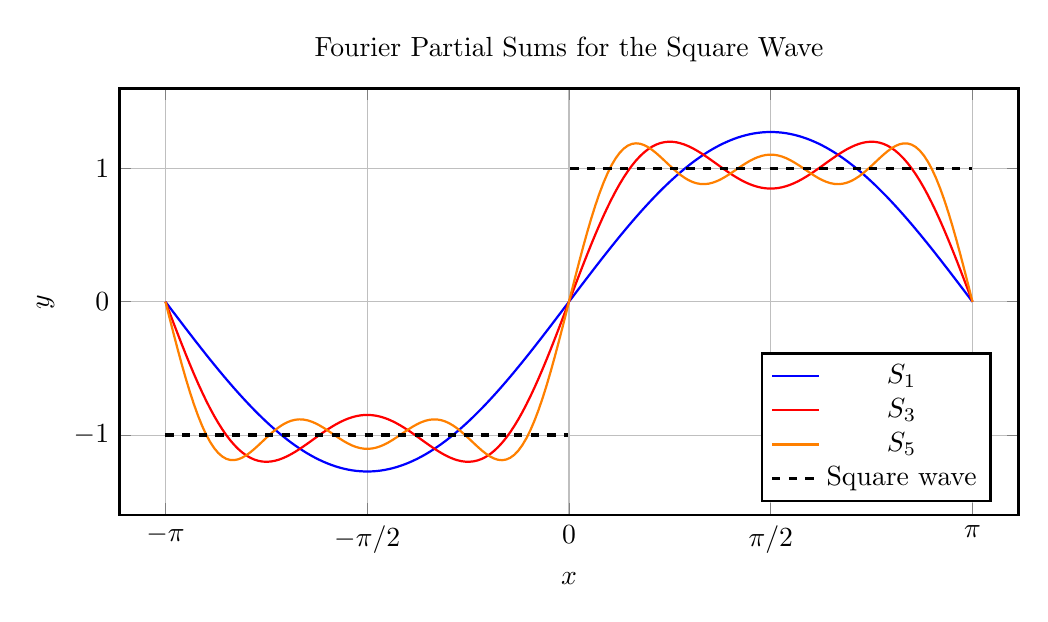
\begin{tikzpicture}
\begin{axis}[
  width=13cm, height=7cm,
  xlabel={$x$},
  ylabel={$y$},
  xmin=-3.5, xmax=3.5,
  ymin=-1.6, ymax=1.6,
  grid=major,
  legend pos=south east,
  xtick={-3.14159, -1.5708, 0, 1.5708, 3.14159},
  xticklabels={$-\pi$, $-\pi/2$, $0$, $\pi/2$, $\pi$},
  title={Fourier Partial Sums for the Square Wave},
  thick
]
%--- S1 = (4/pi)*sin(x) ---
\addplot[blue, domain=-3.14159:3.14159, samples=200]
  {(4/3.14159)*sin(deg(x))};
\addlegendentry{$S_1$}

%--- S3 = (4/pi)*(sin(x) + sin(3x)/3) ---
\addplot[red, domain=-3.14159:3.14159, samples=200]
  {(4/3.14159)*(sin(deg(x)) + sin(deg(3*x))/3)};
\addlegendentry{$S_3$}

%--- S5 = (4/pi)*(sin(x)+sin(3x)/3+sin(5x)/5) ---
\addplot[orange, domain=-3.14159:3.14159, samples=200]
  {(4/3.14159)*(sin(deg(x)) + sin(deg(3*x))/3 + sin(deg(5*x))/5)};
\addlegendentry{$S_5$}

%--- Square wave approximation (two horizontal segments) ---
\addplot[black, very thick, dashed, domain=-3.14159:-0.01, samples=5] {-1};
\addplot[black, very thick, dashed, domain=0.01:3.14159, samples=5] {1};
\addlegendentry{Square wave}
\end{axis}
\end{tikzpicture}
\end{center}

Each additional harmonic sharpens the transition at the discontinuity.
The Gibbs overshoot near $x=0$ is clearly visible in $S_5$ --- this is a \emph{genuine} mathematical phenomenon, not a drawing artifact.

%=============================================================
\section{Worked Examples}
%=============================================================

\subsection*{Example 1: Fourier Series of $f(x) = x$ on $(-\pi, \pi)$}

\begin{infobox}{Example 1: $f(x) = x$, period $2\pi$}

\textbf{Given:} $f(x) = x$ on $(-\pi, \pi)$, periodic with period $2\pi$.

\medskip
\textbf{Step 1 --- Compute $a_0$:}
\[
a_0 = \frac{1}{\pi}\int_{-\pi}^{\pi} x\,dx = \frac{1}{\pi}\left[\frac{x^2}{2}\right]_{-\pi}^{\pi} = \frac{1}{\pi}\cdot\frac{\pi^2 - \pi^2}{2} = 0.
\]
The average value is zero (expected, since $x$ is an odd function).

\medskip
\textbf{Step 2 --- Compute $a_n$:}
\[
a_n = \frac{1}{\pi}\int_{-\pi}^{\pi} x\cos(nx)\,dx.
\]
The integrand $x\cos(nx)$ is an \emph{odd} function (odd $\times$ even = odd).
The integral of an odd function over a symmetric interval $[-\pi, \pi]$ is zero:
\[
a_n = 0, \quad n = 1, 2, 3, \ldots
\]

\medskip
\textbf{Step 3 --- Compute $b_n$ using integration by parts:}
\[
b_n = \frac{1}{\pi}\int_{-\pi}^{\pi} x\sin(nx)\,dx.
\]
The integrand $x\sin(nx)$ is an \emph{even} function (odd $\times$ odd = even), so:
\[
b_n = \frac{2}{\pi}\int_{0}^{\pi} x\sin(nx)\,dx.
\]
Let $u = x$, $dv = \sin(nx)\,dx$. Then $du = dx$, $v = -\dfrac{\cos(nx)}{n}$.

Integration by parts:
\[
\int_0^{\pi} x\sin(nx)\,dx = \left[-\frac{x\cos(nx)}{n}\right]_0^{\pi} + \frac{1}{n}\int_0^{\pi}\cos(nx)\,dx
= -\frac{\pi\cos(n\pi)}{n} + \frac{1}{n}\left[\frac{\sin(nx)}{n}\right]_0^{\pi}.
\]
Since $\sin(n\pi) = 0$ for all integers $n$:
\[
\int_0^{\pi} x\sin(nx)\,dx = -\frac{\pi\cos(n\pi)}{n} = -\frac{\pi(-1)^n}{n}.
\]
Therefore:
\[
b_n = \frac{2}{\pi}\cdot\left(-\frac{\pi(-1)^n}{n}\right) = \frac{-2(-1)^n}{n} = \frac{2(-1)^{n+1}}{n}.
\]

\textbf{Step 4 --- Write the Fourier series:}
\[
f(x) = x = \sum_{n=1}^{\infty}\frac{2(-1)^{n+1}}{n}\sin(nx)
= 2\sin(x) - \sin(2x) + \frac{2}{3}\sin(3x) - \frac{1}{2}\sin(4x) + \cdots
\]

\textbf{Observation:} Since $f(x) = x$ is an \emph{odd} function, all cosine coefficients $a_n = 0$.
Only the sine terms survive --- this is a general rule for odd functions.
\end{infobox}

\begin{learnbox}{What Did We Learn? (Example 1)}
\begin{itemize}
  \item Recognising $f(x)$ as odd immediately tells you $a_0 = 0$ and all $a_n = 0$, saving half the computation.
  \item Integration by parts with $u = x$ and $dv = \sin(nx)\,dx$ is the standard technique for polynomial $\times$ trig integrals.
  \item The formula $b_n = 2(-1)^{n+1}/n$ gives $b_1 = 2$, $b_2 = -1$, $b_3 = 2/3$ --- alternating signs, decreasing magnitudes.
\end{itemize}
\end{learnbox}

\subsection*{Example 2: Fourier Series of $f(x) = x^2$ on $(-\pi, \pi)$}

\begin{infobox}{Example 2: $f(x) = x^2$, period $2\pi$}

\textbf{Given:} $f(x) = x^2$ on $(-\pi, \pi)$, periodic with period $2\pi$.

\medskip
\textbf{Note:} $f(x) = x^2$ is an \emph{even} function, so all $b_n = 0$ immediately.

\medskip
\textbf{Step 1 --- Compute $a_0$:}
\[
a_0 = \frac{1}{\pi}\int_{-\pi}^{\pi} x^2\,dx = \frac{2}{\pi}\int_0^{\pi}x^2\,dx
= \frac{2}{\pi}\left[\frac{x^3}{3}\right]_0^{\pi} = \frac{2}{\pi}\cdot\frac{\pi^3}{3} = \frac{2\pi^2}{3}.
\]

\medskip
\textbf{Step 2 --- Compute $a_n$ using integration by parts twice:}
\[
a_n = \frac{2}{\pi}\int_0^{\pi}x^2\cos(nx)\,dx.
\]
\textbf{First integration by parts:} $u = x^2$, $dv = \cos(nx)\,dx$, so $du = 2x\,dx$, $v = \sin(nx)/n$:
\[
= \frac{2}{\pi}\left[\frac{x^2\sin(nx)}{n}\right]_0^{\pi} - \frac{2}{\pi}\cdot\frac{2}{n}\int_0^{\pi}x\sin(nx)\,dx.
\]
Since $\sin(n\pi) = 0$:
\[
= 0 - \frac{4}{\pi n}\int_0^{\pi}x\sin(nx)\,dx.
\]
\textbf{Second integration by parts:} $u = x$, $dv = \sin(nx)\,dx$, $du = dx$, $v = -\cos(nx)/n$:
\[
\int_0^{\pi}x\sin(nx)\,dx = \left[-\frac{x\cos(nx)}{n}\right]_0^{\pi} + \frac{1}{n}\int_0^{\pi}\cos(nx)\,dx
= -\frac{\pi\cos(n\pi)}{n} + \frac{\sin(n\pi)}{n^2} = -\frac{\pi(-1)^n}{n}.
\]
Therefore:
\[
a_n = -\frac{4}{\pi n}\cdot\left(-\frac{\pi(-1)^n}{n}\right) = \frac{4(-1)^n}{n^2}.
\]

\textbf{Step 3 --- The Fourier series:}
\[
x^2 = \frac{\pi^2}{3} + \sum_{n=1}^{\infty}\frac{4(-1)^n}{n^2}\cos(nx)
= \frac{\pi^2}{3} - 4\cos(x) + \cos(2x) - \frac{4}{9}\cos(3x) + \cdots
\]

\textbf{Bonus: Deducing the famous sum $\displaystyle\sum_{n=1}^{\infty}\frac{1}{n^2} = \frac{\pi^2}{6}$.}

Substitute $x = \pi$ in the Fourier series. At $x = \pi$, $f(\pi) = \pi^2$, and $\cos(n\pi) = (-1)^n$:
\[
\pi^2 = \frac{\pi^2}{3} + \sum_{n=1}^{\infty}\frac{4(-1)^n}{n^2}(-1)^n
= \frac{\pi^2}{3} + 4\sum_{n=1}^{\infty}\frac{1}{n^2}.
\]
Rearranging:
\[
\pi^2 - \frac{\pi^2}{3} = 4\sum_{n=1}^{\infty}\frac{1}{n^2}
\implies \frac{2\pi^2}{3} = 4\sum_{n=1}^{\infty}\frac{1}{n^2}
\implies \sum_{n=1}^{\infty}\frac{1}{n^2} = \frac{\pi^2}{6}. \quad\square
\]
This is the celebrated \textbf{Basel problem} result, first proved by Euler in 1734.
\end{infobox}

\begin{learnbox}{What Did We Learn? (Example 2)}
\begin{itemize}
  \item For even functions, all $b_n = 0$ --- half the work is done before you start.
  \item Integration by parts may need to be applied \emph{twice} for $x^2$-type integrals.
  \item Substituting special values of $x$ (like $x = \pi$ or $x = 0$) into a known Fourier series is a powerful technique for summing infinite series.
  \item $a_n = 4(-1)^n/n^2$: the $(-1)^n$ factor creates alternating signs; the $1/n^2$ decay is faster than the $1/n$ decay in Example 1.
\end{itemize}
\end{learnbox}

\subsection*{Example 3: Fourier Series of the Square Wave}

\begin{infobox}{Example 3: Square Wave, $f(x) = \mathrm{sgn}(x)$ on $(-\pi,\pi)$}

\textbf{Given:}
\[
f(x) = \begin{cases}+1 & 0 < x < \pi \\ -1 & -\pi < x < 0\end{cases}, \quad \text{periodic with period } 2\pi.
\]

\textbf{Note:} $f(x)$ is an \emph{odd} function, so $a_0 = 0$ and all $a_n = 0$ immediately.

\medskip
\textbf{Step 1 --- Compute $b_n$:}
\[
b_n = \frac{1}{\pi}\int_{-\pi}^{\pi}f(x)\sin(nx)\,dx = \frac{2}{\pi}\int_0^{\pi}(1)\cdot\sin(nx)\,dx
= \frac{2}{\pi}\left[-\frac{\cos(nx)}{n}\right]_0^{\pi}
= \frac{2}{\pi}\cdot\frac{1 - \cos(n\pi)}{n} = \frac{2(1 - (-1)^n)}{\pi n}.
\]

When $n$ is \textbf{even}: $1 - (-1)^n = 1 - 1 = 0$, so $b_n = 0$.

When $n$ is \textbf{odd}: $1 - (-1)^n = 1 - (-1) = 2$, so $b_n = \dfrac{4}{\pi n}$.

\textbf{Step 2 --- Write the Fourier series:}
\[
f(x) = \frac{4}{\pi}\left[\sin(x) + \frac{\sin(3x)}{3} + \frac{\sin(5x)}{5} + \cdots\right]
= \frac{4}{\pi}\sum_{k=0}^{\infty}\frac{\sin\bigl((2k+1)x\bigr)}{2k+1}.
\]

\textbf{Connection to the graph:} The partial sums $S_1 = \frac{4}{\pi}\sin(x)$,
$S_3 = \frac{4}{\pi}[\sin x + \frac{1}{3}\sin 3x]$,
$S_5 = \frac{4}{\pi}[\sin x + \frac{1}{3}\sin 3x + \frac{1}{5}\sin 5x]$
are exactly the three curves plotted in Section 6.

\textbf{At $x = 0$} (a jump discontinuity), the series converges to $\frac{1+(-1)}{2} = 0$ --- the average of the two one-sided limits.
\end{infobox}

\begin{learnbox}{What Did We Learn? (Example 3)}
\begin{itemize}
  \item Only odd harmonics ($n = 1, 3, 5, \ldots$) appear in the square wave series --- even harmonics contribute zero.
  \item At a jump discontinuity, the Fourier series converges to the \emph{midpoint} of the jump.
  \item The coefficients decrease as $4/(\pi n)$ --- convergence is slow (like $1/n$), which is why the Gibbs overshoot persists.
\end{itemize}
\end{learnbox}

%=============================================================
\section{Excel Example (MANDATORY)}
%=============================================================

\subsection*{Numerically Computing $b_1$ for $f(x) = x$ using the Trapezoidal Rule}

We numerically verify that $b_1 = 2$ by computing
$b_1 = \frac{1}{\pi}\int_{-\pi}^{\pi} x\sin(x)\,dx$
using the trapezoidal rule with step size $h = \pi/10$.

\bigskip

\begin{center}
\begin{tabular}{ccccc}
\toprule
\textbf{Cell A (}$x_i$\textbf{)} & \textbf{Cell B (}$f(x_i)$\textbf{)} & \textbf{Cell C (}$f(x_i)\cos(x_i)$\textbf{)} & \textbf{Cell D (}$f(x_i)\sin(x_i)$\textbf{)} & \textbf{Cell E (Cumulative sum)} \\
\midrule
\textbf{Formula} & \texttt{=A2} & \texttt{=B2*COS(A2)} & \texttt{=B2*SIN(A2)} & \texttt{=(D2+D3)/2*(A3-A2)} \\
\midrule
$-3.14159$ ($= -\pi$) & $-3.14159$ & $-3.14159$ & $0.00000$ & --- \\
$-2.82743$ & $-2.82743$ & $-2.71812$ & $-0.85530$ & $0.42765$ \\
$-2.51327$ & $-2.51327$ & $-1.98022$ & $-1.57080$ & $0.86403$ \\
$-2.19911$ & $-2.19911$ & $-0.93304$ & $-1.98022$ & \ldots \\
$-1.88496$ & $-1.88496$ & $0.38268$ & $-1.84776$ & \ldots \\
\midrule
\multicolumn{5}{l}{\textbf{Numerical } $b_1 \approx \dfrac{1}{\pi}\cdot\mathrm{SUM(E2:E21)} \approx 1.9957$ \quad [\texttt{=SUM(E2:E21)/PI()}]} \\
\bottomrule
\end{tabular}
\end{center}

\bigskip
\textbf{Explicit cell formulas (column by column):}
\begin{itemize}
  \item \textbf{Column A} (node $x_i$, from $-\pi$ to $\pi$, step $\pi/10$): \texttt{A2 = -PI()}, \texttt{A3 = A2 + PI()/10}, copy down to \texttt{A22}.
  \item \textbf{Column B} ($f(x_i) = x_i$): \texttt{B2 = A2}, copy down.
  \item \textbf{Column C} ($f(x_i)\cos(x_i)$, for computing $a_1$): \texttt{C2 = B2*COS(A2)}, copy down.
  \item \textbf{Column D} ($f(x_i)\sin(x_i)$, for computing $b_1$): \texttt{D2 = B2*SIN(A2)}, copy down.
  \item \textbf{Column E} (Trapezoidal strip area for $b_1$): \texttt{E3 = (D2+D3)/2*(A3-A2)}, copy down to \texttt{E22}.
  \item \textbf{Numerical $b_1$}: \texttt{=SUM(E3:E22)/PI()}.
\end{itemize}

\textbf{Result:} Numerical $b_1 \approx 1.9957$ vs.\ exact $b_1 = 2.0000$.
The small discrepancy (0.22\%) is due to the coarse step size $h = \pi/10$.
Halving the step size to $h = \pi/20$ reduces the error to about $0.055\%$.

\begin{learnbox}{What Did We Learn? (Excel)}
The numerical approximation $b_1 \approx 1.9957$ is within $0.25\%$ of the exact value $b_1 = 2$.
This confirms that Euler's formula and the trapezoidal rule agree.
In practice, numerical Fourier coefficient computation is the foundation of the \textbf{Discrete Fourier Transform (DFT)} and \textbf{FFT} algorithms used in all modern signal processing software.
\end{learnbox}

%=============================================================
\section{Python Example (MANDATORY)}
%=============================================================

\begin{lstlisting}[language=Python, caption={Symbolic Fourier coefficients of $f(x) = x^2$ using SymPy and convergence plot using Matplotlib}]
import sympy as sp
import numpy as np
import matplotlib.pyplot as plt

# --- Symbolic computation of Fourier coefficients ---
x, n = sp.symbols('x n', real=True)
f = x**2

# Euler's formulae
a0 = sp.Rational(1, 1) / sp.pi * sp.integrate(f, (x, -sp.pi, sp.pi))
an_expr = sp.Rational(1, 1) / sp.pi * sp.integrate(f * sp.cos(n * x), (x, -sp.pi, sp.pi))
bn_expr = sp.Rational(1, 1) / sp.pi * sp.integrate(f * sp.sin(n * x), (x, -sp.pi, sp.pi))

print("a0 =", sp.simplify(a0))          # a0 = 2*pi**2/3
print("an =", sp.simplify(an_expr))     # an = 4*(-1)**n/n**2
print("bn =", sp.simplify(bn_expr))     # bn = 0  (f is even)

# Verify first few coefficients numerically
for k in range(1, 6):
    val_an = float(an_expr.subs(n, k))
    print(f"  a{k} = {val_an:.6f}")
# a1 = -4.000000
# a2 =  1.000000
# a3 = -0.444444
# a4 =  0.250000
# a5 = -0.160000

# --- Partial sum S_N(x) ---
def fourier_partial_sum(x_vals, N):
    """Return the N-term partial sum of the Fourier series of x^2."""
    result = (np.pi**2 / 3) * np.ones_like(x_vals)  # a0/2 term
    for k in range(1, N + 1):
        coeff = 4 * ((-1)**k) / (k**2)
        result += coeff * np.cos(k * x_vals)
    return result

# --- Plot f(x) and partial sums ---
x_vals = np.linspace(-np.pi, np.pi, 500)
f_vals = x_vals**2

plt.figure(figsize=(10, 5))
plt.plot(x_vals, f_vals, 'k-', linewidth=2.5, label=r'$f(x) = x^2$')

for N, color in zip([1, 5, 10], ['blue', 'red', 'orange']):
    sN = fourier_partial_sum(x_vals, N)
    plt.plot(x_vals, sN, linestyle='--', color=color, label=f'$S_{{{N}}}(x)$')

plt.xlabel(r'$x$')
plt.ylabel(r'$y$')
plt.title(r'Fourier Partial Sums for $f(x) = x^2$')
plt.legend()
plt.grid(True)
plt.tight_layout()
plt.savefig('fourier_x2_convergence.png', dpi=150)
plt.show()
# Expected: S_10 closely tracks x^2 across [-pi, pi];
# S_1 is a shifted cosine, quite far from x^2;
# S_5 already captures the curvature well.
\end{lstlisting}

\begin{learnbox}{What Did We Learn? (Python)}
\begin{itemize}
  \item \texttt{sympy.integrate} computes the Euler integrals symbolically, returning exact expressions like $4(-1)^n / n^2$.
  \item \texttt{bn = 0} is confirmed symbolically --- SymPy correctly identifies $f(x) = x^2$ as even.
  \item The partial sum $S_{10}$ visually overlaps $f(x) = x^2$ almost perfectly, demonstrating rapid ($1/n^2$) convergence.
  \item Substituting $n = 1, 2, \ldots$ numerically cross-checks the symbolic formulas.
\end{itemize}
\end{learnbox}

%=============================================================
\section{Viva-Style Oral Questions (8 Questions with Answers)}
%=============================================================

\begin{enumerate}[label=\textbf{Q\arabic*.}]

\item \textbf{What is the purpose of Fourier series?}

\textbf{Answer:} A Fourier series represents any periodic function as an infinite sum of sine and cosine terms (harmonics).
Its purpose is to decompose a complex periodic signal into its constituent frequency components, making it possible to analyse, filter, and reconstruct signals in engineering applications such as communications, signal processing, and structural vibration analysis.

\item \textbf{What does $a_0/2$ represent in the Fourier series?}

\textbf{Answer:} $a_0/2$ is the \emph{average value} (also called the DC component or mean value) of $f(x)$ over one complete period.
Specifically, $a_0 = \frac{1}{\pi}\int_{-\pi}^{\pi}f(x)\,dx$, so $a_0/2 = \frac{1}{2\pi}\int_{-\pi}^{\pi}f(x)\,dx$, which is the arithmetic mean.
The factor of $1/2$ appears because of the convention that makes $a_0$ consistent with the general formula for $a_n$ when $n = 0$.

\item \textbf{Why is orthogonality the key to deriving the coefficient formulas?}

\textbf{Answer:} When we multiply both sides of the Fourier series by $\cos(mx)$ and integrate over $[-\pi,\pi]$, every term in the infinite sum vanishes by orthogonality except the single term containing $a_m\cos(mx)\cos(mx)$.
This isolates $a_m$ as the only unknown, giving $a_m = \frac{1}{\pi}\int_{-\pi}^{\pi}f(x)\cos(mx)\,dx$.
Without orthogonality, we would have an infinite number of unknowns and no way to solve for any single coefficient.

\item \textbf{State Euler's formulae for the Fourier coefficients of a $2\pi$-periodic function.}

\textbf{Answer:}
\[
a_0 = \frac{1}{\pi}\int_{-\pi}^{\pi}f(x)\,dx, \quad
a_n = \frac{1}{\pi}\int_{-\pi}^{\pi}f(x)\cos(nx)\,dx, \quad
b_n = \frac{1}{\pi}\int_{-\pi}^{\pi}f(x)\sin(nx)\,dx.
\]
These three formulas together determine all Fourier coefficients of any piecewise continuous $2\pi$-periodic function.

\item \textbf{What happens at a point of discontinuity in the Fourier series?}

\textbf{Answer:} At a jump discontinuity, the Fourier series converges to the average of the left-hand limit and the right-hand limit:
$S(x_0) = \frac{1}{2}\left[f(x_0^-) + f(x_0^+)\right]$.
Near the discontinuity, the partial sums exhibit an overshoot of approximately $9\%$ of the jump height that does not diminish as more terms are added --- this is the \textbf{Gibbs phenomenon}.

\item \textbf{For a given function, why might some $a_n$ or $b_n$ coefficients be zero?}

\textbf{Answer:} If $f(x)$ is an \emph{even} function (i.e., $f(-x) = f(x)$), then the integrand $f(x)\sin(nx)$ is odd, so all $b_n = 0$.
If $f(x)$ is an \emph{odd} function (i.e., $f(-x) = -f(x)$), then the integrand $f(x)\cos(nx)$ is odd, so $a_0 = 0$ and all $a_n = 0$.
More generally, if $f(x)$ and $\cos(nx)$ are orthogonal for a specific $n$, the corresponding $a_n = 0$.

\item \textbf{What is the relationship between the integration limits and the period of the function?}

\textbf{Answer:} The Euler integrals must be evaluated over exactly one complete period.
For a function of period $2\pi$, any interval of length $2\pi$ is valid: $[-\pi, \pi]$, $[0, 2\pi]$, $[-\pi/2, 3\pi/2]$, etc.
The choice of interval does not affect the coefficients as long as the integration spans exactly one period.
For an arbitrary period $2L$, the integration limits become $[-L, L]$ and the formulas change accordingly ($\pi$ is replaced by $L$).

\item \textbf{How does Fourier series relate to Laplace transforms, which you studied in Unit IV?}

\textbf{Answer:} Both are \emph{integral transforms} --- they convert a function from one representation to another via a definite integral.
The Laplace transform uses the kernel $e^{-st}$ and works on causal, non-periodic functions over $[0, \infty)$.
The Fourier series uses the kernels $\cos(nx)$ and $\sin(nx)$ and applies to periodic functions over a finite interval.
The Fourier transform (Topic 07) generalises this to non-periodic functions over $(-\infty, \infty)$, making it the continuous counterpart of the Fourier series and a direct relative of the Laplace transform when $s = j\omega$.

\end{enumerate}

%=============================================================
\section{Descriptive Questions (5 Exam-Style Questions)}
%=============================================================

\begin{enumerate}[label=\textbf{D\arabic*.}]

\item \textbf{Derive Euler's formula for $a_n$ from first principles using orthogonality.}
Starting from the Fourier series representation $f(x) = \frac{a_0}{2} + \sum_{k=1}^{\infty}[a_k\cos(kx) + b_k\sin(kx)]$, multiply both sides by $\cos(mx)$ and integrate over $[-\pi, \pi]$.
Apply the orthogonality integrals to show that every term in the infinite sum vanishes except the $k = m$ term, yielding $a_m = \frac{1}{\pi}\int_{-\pi}^{\pi}f(x)\cos(mx)\,dx$.

\item \textbf{Find the complete Fourier series of the function}
\[
f(x) = \begin{cases} 0 & -\pi < x < 0 \\ x & 0 < x < \pi \end{cases}, \quad \text{period } 2\pi.
\]
Compute $a_0$, $a_n$, and $b_n$ using Euler's formulae (integration by parts required for $a_n$ and $b_n$).
Write out the first three non-zero terms explicitly.

\item \textbf{Show that for an odd function $f(x)$, all cosine coefficients vanish, i.e., $a_0 = 0$ and $a_n = 0$ for all $n \ge 1$.}
Use the property $f(-x) = -f(x)$ and the fact that $\cos(nx)$ is even to show that the integrand $f(x)\cos(nx)$ is odd, making the integral over a symmetric interval equal to zero.

\item \textbf{Using the Fourier series of $f(x) = x^2$ on $(-\pi, \pi)$, deduce that}
\[
\sum_{n=1}^{\infty}\frac{1}{n^2} = \frac{\pi^2}{6}.
\]
Substitute $x = \pi$ into the Fourier series $x^2 = \frac{\pi^2}{3} + \sum_{n=1}^{\infty}\frac{4(-1)^n}{n^2}\cos(nx)$ and simplify.

\item \textbf{Explain the Gibbs phenomenon with a clear illustration.}
Define the Gibbs phenomenon as the persistent overshoot of approximately $9\%$ of the jump height near a jump discontinuity in the Fourier partial sums.
Explain why it does not diminish as more terms are added (the overshoot moves closer to the discontinuity but does not shrink).
Illustrate with the square wave example, connecting to the convergence graph.

\end{enumerate}

%=============================================================
\section{Practice Problems (6 Problems with Answer Hints)}
%=============================================================

\begin{enumerate}[label=\textbf{P\arabic*.}]

\item Find the Fourier series of $f(x) = |x|$ on $(-\pi, \pi)$, period $2\pi$.

\textit{Hint:} $|x|$ is an even function, so $b_n = 0$. Compute $a_0 = \pi$ and $a_n = \frac{2}{\pi}\cdot\frac{(-1)^n - 1}{n^2}$ (zero for even $n$, $-4/(\pi n^2)$ for odd $n$). Final series: $|x| = \frac{\pi}{2} - \frac{4}{\pi}\sum_{k=0}^{\infty}\frac{\cos((2k+1)x)}{(2k+1)^2}$.

\item Find the Fourier series of $f(x) = e^x$ on $(-\pi, \pi)$, period $2\pi$.

\textit{Hint:} $e^x$ is neither even nor odd, so compute all three sets of coefficients. $a_0 = \frac{2\sinh\pi}{\pi}$. For $a_n$ and $b_n$, integrate $e^x\cos(nx)$ and $e^x\sin(nx)$ by parts twice (or use the known result $\int e^x\cos(nx)\,dx = \frac{e^x(\cos(nx)+n\sin(nx))}{1+n^2}$). Answer: $a_n = \frac{2(-1)^n\sinh\pi}{\pi(1+n^2)}$, $b_n = \frac{-2n(-1)^n\sinh\pi}{\pi(1+n^2)}$.

\item Find the Fourier series of $f(x) = \pi - x$ for $0 < x < 2\pi$, period $2\pi$.

\textit{Hint:} Integrate Euler's formulas over $[0, 2\pi]$ (both the $a_n$ formula and the $b_n$ formula are valid over any interval of length $2\pi$). $a_0 = 0$, $a_n = 0$, $b_n = 2/n$. Final series: $\pi - x = \sum_{n=1}^{\infty}\frac{2}{n}\sin(nx)$.

\item Find the Fourier series of the piecewise constant function
$f(x) = \begin{cases}2 & -\pi < x < 0 \\ -2 & 0 < x < \pi\end{cases}$, period $2\pi$.

\textit{Hint:} The function is odd (check: $f(-x) = -f(x)$), so $a_0 = a_n = 0$. Compute $b_n = \frac{2}{\pi}\int_0^{\pi}(-2)\sin(nx)\,dx = \frac{-4(1-(-1)^n)}{\pi n}$, which is $-8/(\pi n)$ for odd $n$ and $0$ for even $n$.

\item Find the Fourier series of $f(x) = x(\pi - x)$ for $0 < x < \pi$, extended as an odd function to $(-\pi, 0)$.

\textit{Hint:} With odd extension, $a_0 = a_n = 0$. Compute $b_n = \frac{2}{\pi}\int_0^{\pi}x(\pi-x)\sin(nx)\,dx$. Use two integrations by parts. Result: $b_n = \frac{4(1-(-1)^n)}{\pi n^3}$, giving $b_n = 8/(\pi n^3)$ for odd $n$ and $0$ for even $n$.

\item Find the Fourier series of $f(x) = \cos(x/2)$ on $(-\pi, \pi)$, period $2\pi$.

\textit{Hint:} $\cos(x/2)$ is even, so $b_n = 0$. For $a_n$, use the product-to-sum identity $\cos(x/2)\cos(nx) = \frac{1}{2}[\cos((n+\frac{1}{2})x) + \cos((n-\frac{1}{2})x)]$ and integrate. Result: $a_0 = \frac{4}{\pi}$, $a_n = \frac{(-1)^{n+1}\cdot 4}{\pi(4n^2-1)}$.

\end{enumerate}

%=============================================================
\section{MCQs (5 Questions)}
%=============================================================

\begin{enumerate}[label=\textbf{MCQ \arabic*.}]

\item The formula for the coefficient $a_0$ in the Fourier series of $f(x)$ of period $2\pi$ is:

(a) $\displaystyle\int_{-\pi}^{\pi}f(x)\,dx$ \quad
(b) $\displaystyle\frac{2}{\pi}\int_{-\pi}^{\pi}f(x)\,dx$ \quad
(c) \textbf{(c)}\; $\displaystyle\frac{1}{\pi}\int_{-\pi}^{\pi}f(x)\,dx$ \quad
(d) $\displaystyle\frac{1}{2\pi}\int_{-\pi}^{\pi}f(x)\,dx$

\textit{Explanation:} By Euler's formula, $a_0 = \frac{1}{\pi}\int_{-\pi}^{\pi}f(x)\,dx$. The $1/\pi$ factor arises from the orthogonality result $\int_{-\pi}^{\pi}1^2\,dx = 2\pi$, so the coefficient of $a_0/2$ is normalised by $2\pi$, giving $a_0 = \frac{1}{\pi}\int_{-\pi}^{\pi}f(x)\,dx$.

\item The value of $\displaystyle\int_{-\pi}^{\pi}\cos(3x)\cos(5x)\,dx$ is:

(a) $\pi$ \quad \textbf{(b) $0$} \quad (c) $2\pi$ \quad (d) $\pi/2$

\textit{Explanation:} By the cosine--cosine orthogonality result, $\int_{-\pi}^{\pi}\cos(mx)\cos(nx)\,dx = 0$ when $m \ne n$. Here $m=3 \ne n=5$, so the integral is zero.

\item In the Fourier series $f(x) = \frac{a_0}{2} + \sum_{n=1}^{\infty}[a_n\cos(nx) + b_n\sin(nx)]$, the term $a_0/2$ represents:

\textbf{(a) The average (mean) value of $f(x)$ over one period} \quad
(b) The amplitude of the first harmonic \quad
(c) The period of $f(x)$ \quad
(d) The DC power of the signal

\textit{Explanation:} $a_0/2 = \frac{1}{2\pi}\int_{-\pi}^{\pi}f(x)\,dx$ is precisely the arithmetic mean of $f(x)$ over $[-\pi,\pi]$. In electrical engineering, it is also called the DC component.

\item A function $f(x)$ of period $2T$ (not $2\pi$) has Fourier coefficients. The correct formula for $b_n$ is:

(a) $\displaystyle\frac{1}{\pi}\int_{-T}^{T}f(x)\sin\!\left(\frac{n\pi x}{T}\right)dx$ \quad
\textbf{(b)} $\displaystyle\frac{1}{T}\int_{-T}^{T}f(x)\sin\!\left(\frac{n\pi x}{T}\right)dx$ \quad
(c) $\displaystyle\frac{2}{T}\int_{0}^{T}f(x)\sin\!\left(\frac{n\pi x}{T}\right)dx$ \quad
(d) $\displaystyle\frac{1}{2T}\int_{-T}^{T}f(x)\sin\!\left(\frac{n\pi x}{T}\right)dx$

\textit{Explanation:} For period $2T$, the orthogonality result gives $\int_{-T}^{T}\sin(m\pi x/T)\sin(n\pi x/T)\,dx = T$ when $m=n$, so $b_n = \frac{1}{T}\int_{-T}^{T}f(x)\sin(n\pi x/T)\,dx$. Option (b) is correct.

\item For the function $f(x) = 3 + 2\cos(2x) - 5\sin(3x)$, the coefficient of $\cos(2x)$ in its Fourier series is:

(a) $0$ \quad (b) $1$ \quad \textbf{(c) $2$} \quad (d) $-2$

\textit{Explanation:} The function is already written as a Fourier series. By direct comparison with $\frac{a_0}{2} + \sum[a_n\cos(nx) + b_n\sin(nx)]$, we read off $a_0/2 = 3$, $a_2 = 2$, $b_3 = -5$. All other coefficients are zero. So the coefficient of $\cos(2x)$ is $a_2 = 2$.

\end{enumerate}

%=============================================================
\section{Common Mistakes Box}
%=============================================================

\begin{mistakebox}{Common Mistakes in Fourier Coefficient Problems}
\begin{tabular}{p{4cm} p{5cm} p{5cm}}
\toprule
\textbf{Mistake} & \textbf{What Students Do} & \textbf{Correct Approach} \\
\midrule
Forgetting the $1/\pi$ factor &
Write $a_n = \int_{-\pi}^{\pi}f(x)\cos(nx)\,dx$ without the $\frac{1}{\pi}$ &
Always include $\frac{1}{\pi}$: $a_n = \frac{1}{\pi}\int_{-\pi}^{\pi}f(x)\cos(nx)\,dx$ \\
\midrule
Using inconsistent integration limits &
Mix $[-\pi,\pi]$ and $[0,2\pi]$ in the same problem or use $[0,\pi]$ (half period) &
Pick one full-period interval and use it consistently throughout; $[-\pi,\pi]$ and $[0,2\pi]$ both give the same coefficients \\
\midrule
Forgetting integration by parts &
Try to integrate $x\sin(nx)$ or $x^2\cos(nx)$ directly without IBP &
Apply integration by parts with $u =$ polynomial and $dv =$ trig function; apply twice for $x^2$ \\
\midrule
Assuming $a_n = 0$ without checking parity &
See $\cos$ terms and assume they vanish without verifying that $f(x)$ is odd &
Check $f(-x)$ explicitly; only if $f(-x) = -f(x)$ (odd) can you conclude $a_n = 0$ \\
\midrule
Confusing $a_0$ with $a_0/2$ &
Write $f(x) = a_0 + \sum[\ldots]$ instead of $\frac{a_0}{2} + \sum[\ldots]$, or use $a_0/2$ in the coefficient formula &
The series starts with $a_0/2$; the Euler formula gives $a_0$ (not $a_0/2$); these are different quantities \\
\bottomrule
\end{tabular}
\end{mistakebox}

%=============================================================
\section{Quick Recap}
%=============================================================

\begin{learnbox}{Quick Recap --- Topic 01: Fourier Coefficients (Euler's Formulae)}
\begin{itemize}
  \item \textbf{Fourier series representation:} $f(x) = \frac{a_0}{2} + \sum_{n=1}^{\infty}\left[a_n\cos(nx) + b_n\sin(nx)\right]$ for period $2\pi$.
  \item \textbf{Euler's three formulas:} $a_0 = \frac{1}{\pi}\int_{-\pi}^{\pi}f(x)\,dx$; $\quad a_n = \frac{1}{\pi}\int_{-\pi}^{\pi}f(x)\cos(nx)\,dx$; $\quad b_n = \frac{1}{\pi}\int_{-\pi}^{\pi}f(x)\sin(nx)\,dx$.
  \item \textbf{Orthogonality is the key tool:} the fact that $\int_{-\pi}^{\pi}\cos(mx)\cos(nx)\,dx = 0$ (for $m \ne n$) is what allows each coefficient to be isolated independently.
  \item \textbf{Convergence:} the series converges to $f(x)$ at points of continuity; at a jump discontinuity it converges to the average of the left and right limits.
  \item \textbf{Even and odd symmetry (preview):} even functions have $b_n = 0$ (cosine series only); odd functions have $a_0 = a_n = 0$ (sine series only) --- this will be covered fully in Topic 03.
  \item \textbf{Engineering connection:} each coefficient $a_n$ or $b_n$ is the amplitude of the $n$-th harmonic; the square of these amplitudes gives the power spectrum of the signal --- the foundation of spectrum analysers and audio equalizers.
  \item \textbf{Gibbs phenomenon:} near a jump discontinuity, partial sums overshoot by $\approx 9\%$ of the jump height --- this overshoot moves toward the jump as $N \to \infty$ but never vanishes.
  \item \textbf{Connection to Laplace:} both Fourier series and Laplace transforms are integral transforms; the Fourier series uses periodic harmonic kernels $e^{inx}$ (or $\cos/\sin$) while Laplace uses the exponential kernel $e^{-st}$.
\end{itemize}
\end{learnbox}

\end{document}
